\documentclass[11pt,a4paper]{article}
\usepackage[utf8]{inputenc}
\usepackage[T1]{fontenc}
\usepackage[spanish,es-noshorthands]{babel}
\usepackage{lmodern}
\usepackage[margin=2.4cm]{geometry}
\usepackage{graphicx}
\usepackage{booktabs}
\usepackage{longtable}
\usepackage{array}
\usepackage{hyperref}
\usepackage{xcolor}
\usepackage{amsmath}
\usepackage{enumitem}

\graphicspath{{../results/etapa2/figures/}{../results/etapa2/confusion_matrices/}}
\hypersetup{colorlinks=true, linkcolor=blue!45!black, urlcolor=blue!45!black}
\setlength{\parskip}{0.35em}
\setlength{\parindent}{0pt}
\setlength{\emergencystretch}{3em}
\addto\captionsspanish{\renewcommand{\tablename}{Tabla}}
\renewcommand{\arraystretch}{1.15}
\newcommand{\code}[1]{\texttt{#1}}

\begin{document}

\begin{titlepage}
\centering
\vspace*{2.2cm}
{\Large Proyecto Etapa II}\\[0.5cm]
{\Huge\bfseries Clasificación y clustering\\[0.2cm] de artículos científicos}\\[1.2cm]
{\large Aprendizaje automático tradicional aplicado a NLP}\\[2.2cm]
\begin{tabular}{rl}
\textbf{Equipo:} & Angel Garcia · Bren\\[0.2cm]
\textbf{Entrega:} & 17 de noviembre de 2026\\
\end{tabular}
\vfill
{\small Repositorio: \code{PracticaML} · Corpus: 500 artículos de arXiv}
\end{titlepage}

\tableofcontents
\newpage

\section*{Resumen}
\addcontentsline{toc}{section}{Resumen}

Este trabajo extiende el buscador de artículos científicos de la Etapa I con dos tareas
de aprendizaje automático tradicional: clasificación supervisada de la categoría primaria
de arXiv (tarea A, obligatoria) y clustering con K-Means (tarea B, elegida). Se reutilizan
los 500 artículos del corpus, sus identificadores y el benchmark congelado, sin usar LLM
ni modelos generativos.

La clasificación se resolvió con \emph{Pipelines} de scikit-learn, búsqueda de
hiperparámetros solo en train y selección por macro-F1 en dev. La mejor configuración fue
LogisticRegression con normalización N2, TF-IDF de unigramas y \code{min\_df=1}: macro-F1
0.799 en dev y 0.761 en test. TF-IDF superó a las representaciones binaria y de frecuencia;
la lematización ayudó a MultinomialNB; los bigramas, los trigramas y el SVD no aportaron
mejoras materiales a LR. En SVC, SVD 50 subió 1.4 puntos en dev pero con CV menor y se
añadió después de congelar la selección, así que no se usó en test. El análisis de 10
errores de dev muestra que la frontera
\code{cs.CL}--\code{cs.LG}, el vocabulario de recuperación y la etiqueta primaria de arXiv
explican la mayor parte de las confusiones.

K-Means se ajustó sin etiquetas y se evaluó con silhouette, estabilidad y interpretabilidad.
La configuración final (k=4, N2, TF-IDF, SVD 100) obtuvo silhouette 0.083 en test, ARI 0.372
y NMI 0.486; sus cuatro clusters se leen como NLP/agentes, IR/recomendación,
visión/vídeo y ML general. Un resultado relevante es que las configuraciones con silhouette
más alto (texto crudo, frecuencia, bigramas, SVD 50) separaban artefactos de formato
(números y LaTeX), no áreas de investigación; por eso la selección final combinó silhouette
en dev con interpretabilidad, tal como advierte el enunciado.

\newpage
\section{Introducción}

La Etapa I construyó un buscador de artículos científicos basado en el modelo de espacio
vectorial: 500 artículos de arXiv de cuatro categorías (\code{cs.CL}, \code{cs.CV},
\code{cs.IR}, \code{cs.LG}), 12 configuraciones de recuperación, un benchmark de 15
consultas y una interfaz web y de línea de comandos. La Etapa II pide comparar
sistemáticamente pipelines clásicos de NLP sobre esa misma colección, sin modelos
generativos, documentando normalización, representación, hiperparámetros, selección en dev
y evaluación final en test.

El proyecto tiene dos tareas:
\begin{itemize}[leftmargin=1.4em]
\item \textbf{Tarea A (obligatoria):} clasificación supervisada de la categoría primaria.
\item \textbf{Tarea B (opcional, elegida):} clustering de documentos con K-Means.
\end{itemize}

Las contribuciones principales son: (i) una partición reproducible 70/15/15 fijada antes
de ajustar cualquier transformación; (ii) 29 experimentos de clasificación y 17 de
clustering registrados en \code{experiments.tsv}; (iii) los entregables de predicciones,
métricas por clase, matrices de confusión y clusters; (iv) una interfaz de consulta; y
(v) este informe, con análisis de errores y limitaciones.

\section{Corpus y etiquetas}

\subsection{Corpus}
Se reutiliza \code{data/scientific\_raw\_corpus.tsv} de la Etapa I sin ampliarlo: 500
artículos, 125 por categoría. La entrada del modelo es la concatenación
$X = \text{título} + ". " + \text{abstract}$. El identificador \code{document\_id} es el
\code{arxiv\_id} leído como texto, para no perder ceros iniciales.

\subsection{Política de etiqueta}
La etiqueta $y$ es \code{primary\_category}, la categoría primaria que asigna arXiv. Se
verificó que \code{primary\_category} coincide con el primer elemento de \code{categories}
en los 500 documentos, que no hay etiquetas vacías ni identificadores duplicados. Las
categorías secundarias (cross-listing) se conservan como metadato y no se usan como
etiqueta; sirven para explicar errores.

\begin{table}[htbp]
\centering
\small
\caption{Distribución de clases y cross-listing.}
\label{tab:clases}
\begin{tabular}{@{}lrr@{}}
\toprule
Clase & Documentos & \% con categoría secundaria\\
\midrule
\code{cs.CL} & 125 & 56.0\\
\code{cs.CV} & 125 & 43.2\\
\code{cs.IR} & 125 & 43.2\\
\code{cs.LG} & 125 & 59.2\\
\midrule
Total & 500 & 50.4\\
\bottomrule
\end{tabular}
\end{table}

El cross-listing es alto: entre 43\,\% y 59\,\% de los artículos tienen al menos una
categoría secundaria. Esto anticipa que las fronteras entre clases no son nítidas y que
parte de los errores del clasificador serán estructurales, no de ajuste.

\begin{figure}[htbp]
\centering
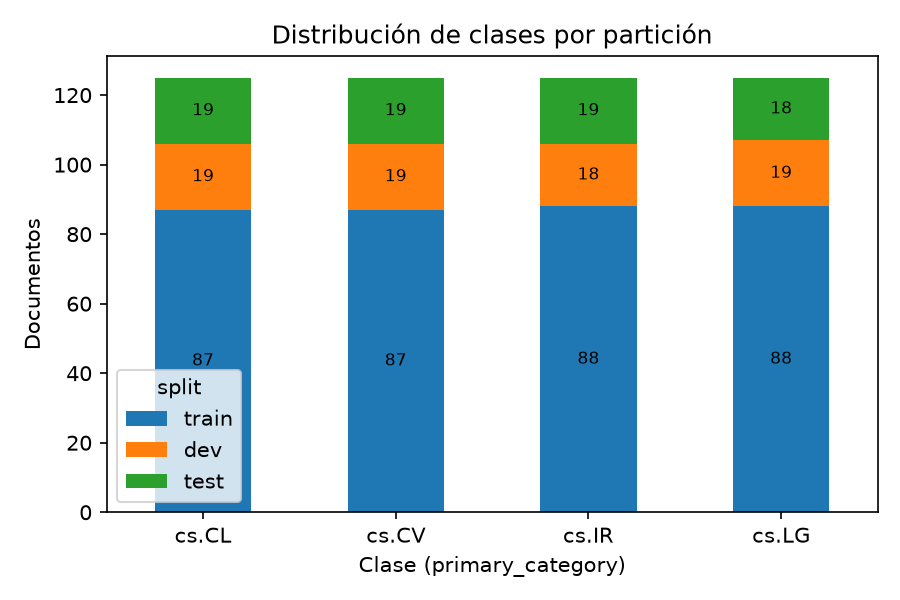
\includegraphics[width=0.62\linewidth]{class_distribution.png}
\caption{Distribución de clases por partición.}
\label{fig:distribucion}
\end{figure}

\section{Particiones y control de fuga}

Los splits se fijaron \textbf{antes} de ajustar vectorizadores, SVD o modelos, con dos
cortes estratificados de \code{train\_test\_split} (\code{shuffle=True},
\code{random\_state=0}): 70/30 y después 30 en 15/15. El resultado es 350 documentos de
train, 75 de dev y 75 de test, con las cuatro clases presentes en las tres particiones
(Tabla~\ref{tab:splits}).

\begin{table}[htbp]
\centering
\small
\caption{Documentos por clase y partición.}
\label{tab:splits}
\begin{tabular}{@{}lrrr@{}}
\toprule
Clase & Train & Dev & Test\\
\midrule
\code{cs.CL} & 87 & 19 & 19\\
\code{cs.CV} & 87 & 19 & 19\\
\code{cs.IR} & 88 & 18 & 19\\
\code{cs.LG} & 88 & 19 & 18\\
\midrule
Total & 350 & 75 & 75\\
\bottomrule
\end{tabular}
\end{table}

Todo lo que aprende de los datos (vocabulario, IDF, SVD, modelo) está dentro de un
\code{Pipeline} y se ajusta solo con train. La normalización se precalcula porque es una
transformación documento a documento que no aprende del corpus; aun así, dentro del
\code{Pipeline} un transformador \code{NormalizedText} recupera el texto ya normalizado,
de modo que train, dev y test pasan por el mismo camino. Test se reservó para una única
evaluación final.

Con 75 documentos en dev, un documento equivale a unos 1.3 puntos de accuracy o macro-F1.
Por eso el proyecto reporta también el macro-F1 de la validación cruzada en train y trata
las diferencias menores a un punto como no concluyentes.

\section{Normalización}

Se compararon tres configuraciones, incluida una línea base mínima:

\begin{table}[htbp]
\centering
\small
\caption{Configuraciones de normalización y tamaño del vocabulario en train.}
\label{tab:norm}
\begin{tabular}{@{}p{1.1cm}p{7.4cm}rr@{}}
\toprule
ID & Operaciones & Tokens/doc & Vocab. train\\
\midrule
N0 & Tokenización con spaCy; conserva mayúsculas y puntuación & 257.8 & 9\,974\\
N1 & N0 + minúsculas, sin puntuación ni stopwords (\code{is\_stop}) & 145.1 & 8\,098\\
N2 & Normalización de la Etapa I: minúsculas, lemas y filtro POS
(DET, ADP, CCONJ, SCONJ, PRON, AUX) & 155.7 & 6\,689\\
\bottomrule
\end{tabular}
\end{table}

N2 es la normalización de la Etapa I y la que deja el vocabulario más compacto.
N1 elimina más tokens porque \code{is\_stop} quita más palabras que el filtro por POS,
pero no une formas de una misma palabra; N2 sí lo hace mediante la lematización.
El vectorizador usa un tokenizador por espacios, \code{lowercase=False} y
\code{token\_pattern=None}: si volviera a pasar a minúsculas y a quitar puntuación, N0
quedaría igual que N1 y el experimento de normalización no mediría nada.

\section{Representaciones y diseño experimental}

\subsection{Representaciones y modelos}
Se compararon tres representaciones: binaria (\code{CountVectorizer(binary=True)}),
frecuencia (\code{CountVectorizer()}) y TF-IDF. Los n-gramas fueron (1,1), (1,2) y (1,3).
El SVD se probó con 50, 100 y 200 componentes, siempre dentro del \code{Pipeline}. Los
clasificadores fueron MultinomialNB, LogisticRegression y SVC lineal. MultinomialNB nunca
se combinó con SVD porque el SVD produce valores negativos.

Los hiperparámetros se buscaron con \code{GridSearchCV} y
\code{StratifiedKFold(5, shuffle=True, random\_state=0)}, con \code{scoring="f1\_macro"},
solo sobre train. La rejilla fue \code{min\_df} $\in \{1,2\}$ y \code{alpha} $\in
\{0.1,0.5,1.0\}$ para NB, o $C \in \{0.1,1,10\}$ para LR y SVC. Cada experimento es un
\code{Pipeline} completo; dev solo evalúa el mejor estimador.

\subsection{Bloques}
El diseño cambia un factor a la vez y arrastra la mejor opción del bloque anterior por
modelo (Tabla~\ref{tab:bloques}). Los experimentos de clasificación se numeran C01--C25;
los de clustering, K01--K16.

\begin{table}[htbp]
\centering
\footnotesize
\caption{Bloques de experimentos.}
\label{tab:bloques}
\begin{tabular}{@{}>{\raggedright\arraybackslash}p{1.2cm}>{\raggedright\arraybackslash}p{4.0cm}>{\raggedright\arraybackslash}p{3.8cm}>{\raggedright\arraybackslash}p{4.4cm}@{}}
\toprule
Bloque & Factor que cambia & Fijo & Experimentos\\
\midrule
C-1 & Clasificador: NB, LR, SVC & N2, TF-IDF (1,1), sin SVD & C01--C03\\
C-2 & Normalización: N0, N1, N2 & TF-IDF (1,1), sin SVD & C01--C09\\
C-3 & Representación: binaria, frecuencia, TF-IDF & mejor normalización por modelo & C02, C06, C07, C10--C15\\
C-4 & N-gramas: (1,1), (1,2), (1,3) & mejor representación & C02, C06, C07, C16--C21\\
C-5 & SVD: 50, 100, 200 & mejor configuración y configuración final & C22--C29\\
\midrule
K-1 & $k \in \{3,4,5,6,8\}$ & N2, TF-IDF (1,1), SVD 100 & K01--K05\\
K-2 & Normalización & mejor $k$ & K01, K06, K07\\
K-3 & Binaria, frecuencia, TF-IDF & mejor normalización & K08, K17 + referencia\\
K-4 & (1,1) vs (1,2) & mejor representación & K09 + referencia\\
K-5 & SVD: sin SVD, 50, 100, 200 & mejor configuración & K10--K12 + referencia\\
K-6 & \code{init}, \code{n\_init}, \code{max\_iter} & mejor configuración & K13--K16 + referencia\\
\bottomrule
\end{tabular}
\end{table}

\subsection{Criterio de selección}
La métrica primaria de clasificación es el macro-F1 en dev. Si la diferencia con el
siguiente candidato es menor que un punto (0.01 en la escala 0--1, menos de un documento
en dev), se considera empate y se desempata por el macro-F1 de la validación cruzada y por
la configuración más simple (sin SVD y con n-gramas más cortos). Para K-Means el criterio
fue silhouette en dev, estabilidad con cinco semillas e interpretabilidad, en ese orden,
con la salvedad de que el silhouette solo se compara dentro del mismo espacio de
características.

\section{Clasificación: resultados}

\subsection{Clasificadores y normalización}
El bloque C-1 fijó N2, TF-IDF y unigramas. LogisticRegression fue el mejor en dev
(0.799), seguido de MultinomialNB (0.761) y SVC (0.748); en la validación cruzada las
diferencias fueron menores a dos puntos. El bloque C-2 mostró que la normalización importa
de forma desigual: NB mejoró 7 puntos al pasar de N0 a N1, LR mejoró 4 puntos de N0 a N2 y
SVC prácticamente no cambió en CV (Tabla~\ref{tab:c1c2}).

\begin{table}[htbp]
\centering
\small
\caption{C-1 y C-2: macro-F1 en dev y CV.}
\label{tab:c1c2}
\begin{tabular}{@{}llrrr@{}}
\toprule
Modelo & Normalización & Exp. & Dev macro-F1 & CV macro-F1\\
\midrule
MultinomialNB & N2 & C01 & 0.7607 & 0.7594\\
MultinomialNB & N1 & C07 & 0.7745 & 0.7612\\
MultinomialNB & N0 & C04 & 0.7046 & 0.7306\\
\midrule
LogisticRegression & N2 & C02 & 0.7993 & 0.7675\\
LogisticRegression & N1 & C08 & 0.7981 & 0.7486\\
LogisticRegression & N0 & C05 & 0.7602 & 0.7442\\
\midrule
SVC & N2 & C03 & 0.7481 & 0.7478\\
SVC & N1 & C09 & 0.7613 & 0.7487\\
SVC & N0 & C06 & 0.7742 & 0.7451\\
\bottomrule
\end{tabular}
\end{table}

\subsection{Representación, n-gramas y SVD}
TF-IDF ganó en los tres modelos (Tabla~\ref{tab:c3c5}). La representación binaria y la de
frecuencia perdieron entre 3 y 9 puntos, sobre todo en SVC con frecuencia (0.662). Una
explicación plausible es que TF-IDF baja el peso de términos presentes en casi todos los
abstracts y sube el de los que distinguen un área.

\begin{table}[htbp]
\centering
\small
\caption{C-3, C-4 y C-5: macro-F1 en dev de las configuraciones nuevas.}
\label{tab:c3c5}
\footnotesize
\begin{tabular}{@{}llrrrr@{}}
\toprule
Modelo & Alternativa & Exp. & Dev macro-F1 & CV macro-F1 & ¿Mejora?\\
\midrule
MultinomialNB & binaria & C10 & 0.7049 & 0.7404 & no\\
MultinomialNB & frecuencia & C11 & 0.7327 & 0.7492 & no\\
MultinomialNB & bigramas & C16 & 0.7673 & 0.7500 & no\\
MultinomialNB & trigramas & C17 & 0.7554 & 0.7539 & no\\
\midrule
LogisticRegression & binaria & C12 & 0.7445 & 0.7437 & no\\
LogisticRegression & frecuencia & C13 & 0.7457 & 0.7326 & no\\
LogisticRegression & bigramas & C18 & 0.8007 & 0.7656 & empate\\
LogisticRegression & trigramas & C19 & 0.7751 & 0.7672 & no\\
LogisticRegression & SVD 100 (C18) & C22 & 0.7573 & 0.7654 & no\\
LogisticRegression & SVD 200 (C18) & C23 & 0.7713 & 0.7849 & no\\
LogisticRegression & SVD 50 (C02) & C28 & 0.7706 & 0.7411 & no\\
LogisticRegression & SVD 100 (C02) & C26 & 0.7586 & 0.7601 & no\\
LogisticRegression & SVD 200 (C02) & C27 & 0.7475 & 0.7653 & no\\
\midrule
SVC & binaria & C14 & 0.7466 & 0.7081 & no\\
SVC & frecuencia & C15 & 0.6624 & 0.6532 & no\\
SVC & bigramas & C20 & 0.7458 & 0.7386 & no\\
SVC & trigramas & C21 & 0.7566 & 0.7218 & no\\
SVC & SVD 50 (C06) & C29 & 0.7880 & 0.7040 & sí en dev\\
SVC & SVD 100 (C06) & C24 & 0.7504 & 0.7319 & no\\
SVC & SVD 200 (C06) & C25 & 0.7751 & 0.7302 & empate\\
\bottomrule
\end{tabular}
\end{table}

Los bigramas y trigramas no aportaron una mejora material. LR con bigramas obtuvo 0.8007
frente a 0.7993 de unigramas (0.0014, una décima de documento) y con trigramas bajó a
0.7751; NB y SVC empeoraron. El SVD no ayudó a LR: sobre la configuración de C-4 (bigramas,
C18) dio 0.7573 con 100 componentes y 0.7713 con 200; sobre la configuración final C02
(unigramas) dio 0.7706 con 50, 0.7586 con 100 y 0.7475 con 200, todos por debajo de
0.7993. En SVC, SVD 100/200 quedó en 0.7504/0.7751; el complemento con SVD 50 (C29) subió
a 0.7880 en dev (+1.4 puntos, poco más de un documento), pero su CV bajó a 0.7040 frente a
0.7451 de C06. C29 se añadió después de congelar la selección y de evaluar test; por el
protocolo de test único no se re-evaluó, así que se mantiene C06 como SVC de referencia y
C29 queda como línea para un test independiente.

\subsection{Selección en dev y evaluación final}
La Tabla~\ref{tab:seleccion} resume el mejor experimento de cada modelo. En LR, C18
(0.8007) y C02 (0.7993) están empatados; se eligió C02 por mayor CV (0.7675 frente a
0.7656) y por ser más simple (unigramas). En SVC, C25 (0.7751) y C06 (0.7742) también
están empatados; se eligió C06 por mayor CV (0.7451 frente a 0.7302) y por no usar SVD. El
ganador global fue C02. El complemento C29 (SVC + SVD 50) llegó a 0.7880 en dev, por
encima de C06, pero se añadió después de congelar la selección y de evaluar test; con CV
0.7040 frente a 0.7451 se mantiene C06. C29 queda como línea para un test independiente.

\begin{table}[htbp]
\centering
\small
\caption{Configuración seleccionada por clasificador y evaluación final (la selección se congeló antes de test).}
\label{tab:seleccion}
\begin{tabular}{@{}llrrr@{}}
\toprule
Modelo & Configuración & Exp. & Dev macro-F1 & Test macro-F1\\
\midrule
MultinomialNB & N1, TF-IDF (1,1), alpha=0.1, min\_df=2 & C07 & 0.7745 & --\\
LogisticRegression & N2, TF-IDF (1,1), C=1, min\_df=1 & C02 & 0.7993 & \textbf{0.7610}\\
SVC & N0, TF-IDF (1,1), C=10, min\_df=1 & C06 & 0.7742 & --\\
\bottomrule
\end{tabular}
\end{table}

Solo el ganador global se reajustó con train+dev (425 documentos) y se evaluó una vez en
test. Los resultados finales se muestran en la Tabla~\ref{tab:test}. La exactitud fue
0.760 y el macro-F1 0.761; el descenso respecto a dev (0.799) es de 3.8 puntos, algo
esperable con 75 documentos y una selección que ya había visto dev.

\begin{table}[htbp]
\centering
\small
\caption{Métricas finales en test del ganador global (C02, LogisticRegression).}
\label{tab:test}
\begin{tabular}{@{}lrrrr@{}}
\toprule
Split & Accuracy & Macro precisión & Macro recall & Macro-F1\\
\midrule
Test & 0.760 & 0.768 & 0.762 & 0.761\\
\bottomrule
\end{tabular}
\end{table}

\begin{table}[htbp]
\centering
\small
\caption{Métricas por clase en test.}
\label{tab:testclase}
\begin{tabular}{@{}lrrrr@{}}
\toprule
Clase & Precisión & Recall & F1 & Soporte\\
\midrule
\code{cs.CL} & 0.579 & 0.579 & 0.579 & 19\\
\code{cs.CV} & 0.875 & 0.737 & 0.800 & 19\\
\code{cs.IR} & 0.889 & 0.842 & 0.865 & 19\\
\code{cs.LG} & 0.727 & 0.889 & 0.800 & 18\\
\bottomrule
\end{tabular}
\end{table}

\begin{figure}[htbp]
\centering
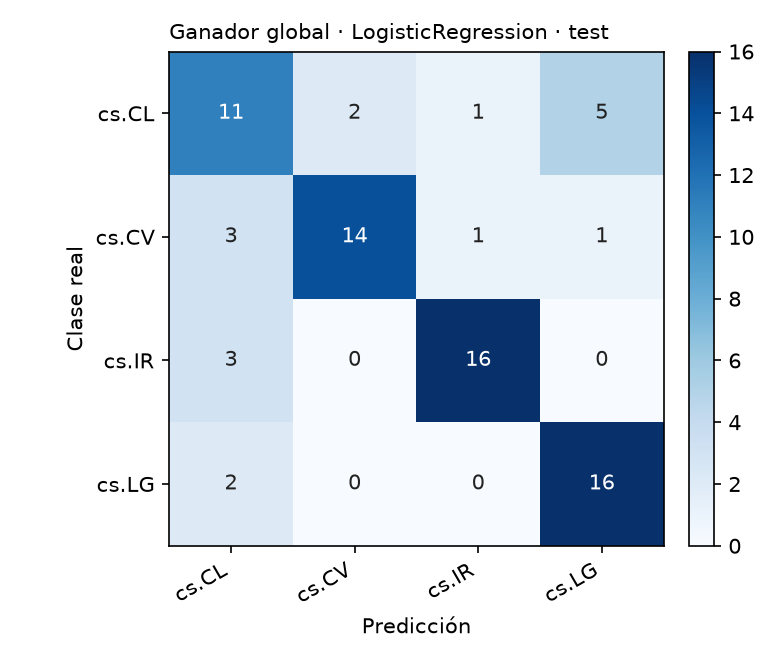
\includegraphics[width=0.55\linewidth]{test.png}
\caption{Matriz de confusión en test del ganador global.}
\label{fig:confusiontest}
\end{figure}

\textbf{Lectura.} \code{cs.CL} es la clase más difícil: F1 0.579, con 5 documentos que se
van a \code{cs.LG}, 2 a \code{cs.CV} y 1 a \code{cs.IR}. \code{cs.CV} y \code{cs.IR}
alcanzan 0.800 y 0.865; \code{cs.LG} llega a 0.800 pero pierde 2 documentos a
\code{cs.CL}. La confusión \code{cs.CL}--\code{cs.LG} es la misma que aparecía en dev y en
el cross-listing. El descenso de dev a test se concentra en CL: en dev su F1 era 0.703 y
en test 0.579.

\begin{figure}[htbp]
\centering
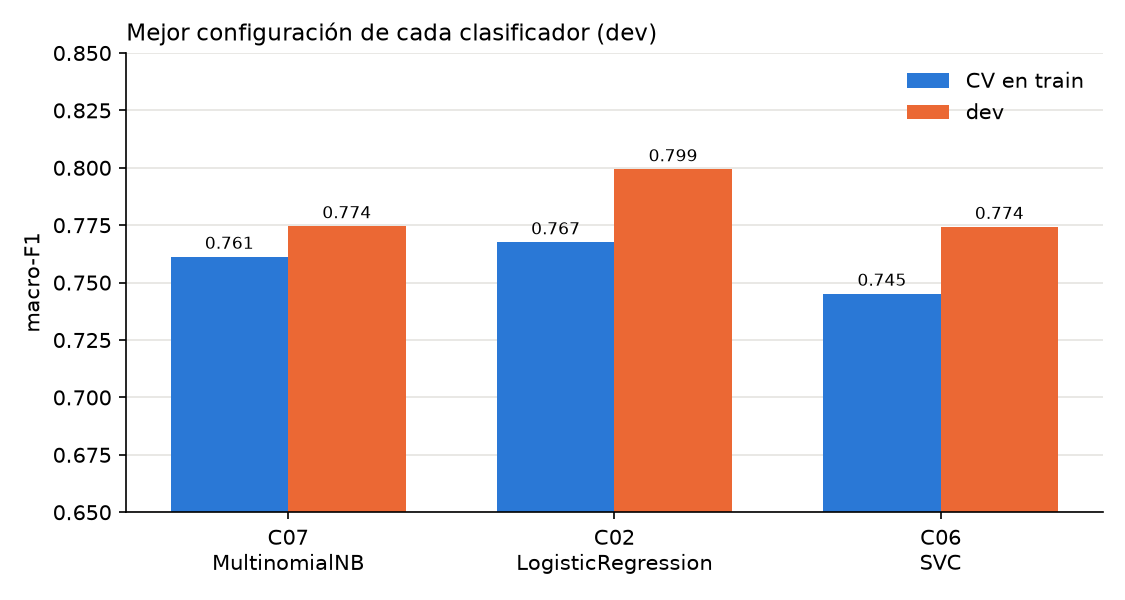
\includegraphics[width=0.78\linewidth]{classification_best_dev.png}
\caption{Mejor configuración de cada clasificador en dev.}
\label{fig:mejores}
\end{figure}

\begin{figure}[htbp]
\centering
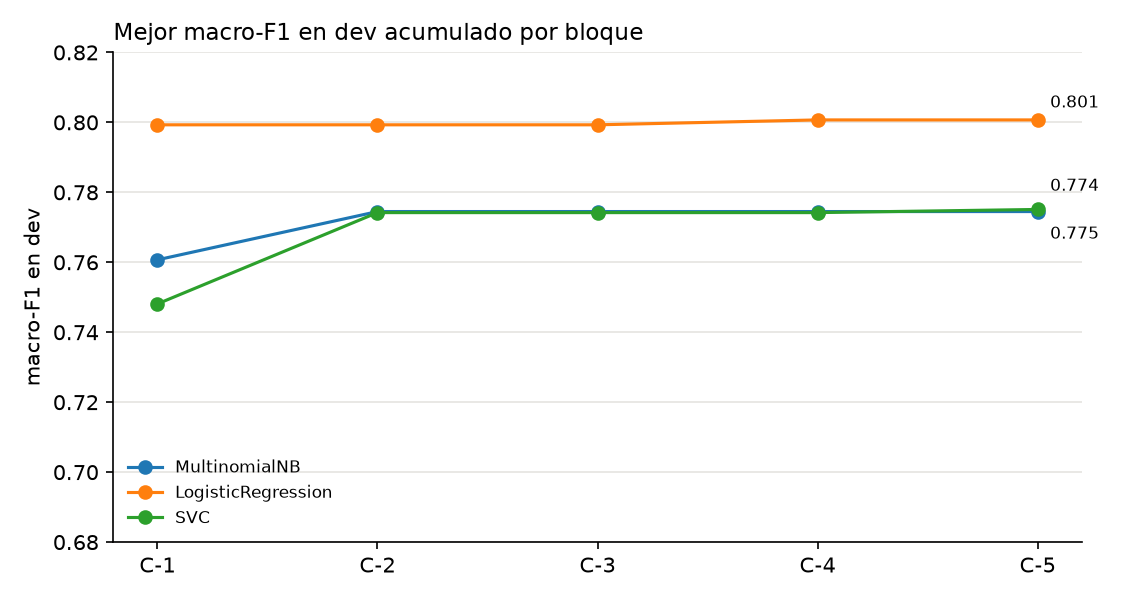
\includegraphics[width=0.78\linewidth]{classification_blocks_dev.png}
\caption{Mejor macro-F1 en dev acumulado por bloque (experimentos originales C01--C25; el complemento C26--C29 se detalla en la Tabla~\ref{tab:c3c5}).}
\label{fig:bloques}
\end{figure}

\section{Análisis de errores}

Se revisaron los errores de dev de C02, el modelo ajustado solo con train (15 errores de
75, 20\,\%). Solo 3 de los 15 errores tienen la clase predicha dentro del cross-listing
del artículo; el resto se explica por solapamiento de vocabulario y por la ambigüedad de
la etiqueta primaria.

\begin{table}[htbp]
\centering
\small
\caption{Pares de confusión en dev (C02).}
\label{tab:pares}
\begin{tabular}{@{}llr@{}}
\toprule
Gold & Predicho & Documentos\\
\midrule
\code{cs.CL} & \code{cs.IR} & 3\\
\code{cs.CV} & \code{cs.CL} & 3\\
\code{cs.CL} & \code{cs.LG} & 2\\
\code{cs.LG} & \code{cs.CL} & 2\\
\code{cs.CL} & \code{cs.CV} & 1\\
\code{cs.CV} & \code{cs.LG} & 1\\
\code{cs.IR} & \code{cs.LG} & 1\\
\code{cs.LG} & \code{cs.CV} & 1\\
\code{cs.LG} & \code{cs.IR} & 1\\
\bottomrule
\end{tabular}
\end{table}

\begin{longtable}{@{}p{1.9cm}p{2.3cm}p{2.3cm}>{\raggedright\arraybackslash}p{7.2cm}@{}}
\caption{Los 10 documentos de dev revisados (detalle completo en
\code{results/etapa2/error\_analysis.md}).}\\
\toprule
ID & Gold & Predicho & Causa probable\\
\midrule
\endfirsthead
\toprule
ID & Gold & Predicho & Causa probable\\
\midrule
\endhead
2609.39460 & \code{cs.CL} & \code{cs.CV} & Error de generalización: el abstract es de lingüística computacional, pero acumula vocabulario de evaluación de clasificadores (\emph{dataset}, \emph{ROC-AUC}, \emph{classifiers}) y pocos términos de NLP.\\
2610.06902 & \code{cs.CL} & \code{cs.IR} & Cross-listing: el artículo también está listado en \code{cs.IR}; habla de recuperación jerárquica para QA.\\
2609.39982 & \code{cs.CL} & \code{cs.LG} & Frontera LLM/ML: agentes de terminal, generación estocástica y cómputo en test.\\
2610.00825 & \code{cs.CV} & \code{cs.CL} & Visión-lenguaje: juez multimodal de lip-sync para doblaje.\\
2609.40222 & \code{cs.CV} & \code{cs.LG} & \emph{World models} de vídeo: mezcla atención, memoria y transformers (LG) con escenas y cámara (CV).\\
2609.28383 & \code{cs.IR} & \code{cs.LG} & Predicción de \emph{watch time} y ranking: vocabulario de recomendación y de ML.\\
2610.00767 & \code{cs.LG} & \code{cs.CL} & Cross-listing: el artículo también está en \code{cs.CL}; intervenciones de preentrenamiento y creencias del modelo.\\
2610.02251 & \code{cs.LG} & \code{cs.CV} & Muestreo especulativo para difusión: evalúa generación en píxeles (FFHQ, CIFAR-10, difusión latente).\\
2610.02249 & \code{cs.LG} & \code{cs.IR} & Usa \emph{retrieval} de vecinos cercanos; el vocabulario de búsqueda y benchmarking pesa aunque la tarea sea predicción molecular.\\
2609.38861 & \code{cs.CL} & \code{cs.IR} & Cross-listing: el artículo también está en \code{cs.IR}; recuperación de evidencia y QA sobre literatura.\\
\bottomrule
\end{longtable}

\textbf{Lecciones.} Los errores se concentran en tres fronteras: \code{cs.CL}--\code{cs.LG}
(LLM y ML comparten transformer, training, model, language), \code{cs.CV}--\code{cs.CL}
(modelos visión-lenguaje) y \code{cs.CL}--\code{cs.IR} (RAG y recuperación). El
cross-listing explica solo una parte; la otra es solapamiento real de vocabulario. La
etiqueta primaria de arXiv es una convención: un artículo de NLP que usa recuperación
puede ser legítimamente \code{cs.CL} o \code{cs.IR}, y el modelo no tiene forma de saber
cuál eligió el autor. Estos errores son esperables con 500 documentos y no se corrigieron
mirando test.

\section{Clustering con K-Means}

\subsection{Diseño}
El pipeline fue \code{NormalizedText} $\rightarrow$ vectorizador $\rightarrow$
\code{TruncatedSVD} (opcional) $\rightarrow$ \code{Normalizer} $\rightarrow$ \code{KMeans}.
K-Means se ajustó solo con train y sin etiquetas; las etiquetas se usaron después, solo
para ARI/NMI y la tabla de contingencia. El silhouette se calculó con distancia coseno en
el espacio SVD+L2 (o en el espacio del vectorizador si no hay SVD), y se declara en cada
tabla. La estabilidad se midió con cinco semillas (0--4) y el ARI entre las particiones
resultantes. Las palabras principales se obtuvieron en el espacio original de palabras con
un vocabulario de contenido (palabras alfabéticas de 4+ letras, \code{min\_df=5},
\code{max\_df=0.5}, sin stopwords), y los documentos representativos son los dos más
cercanos al centroide de cada cluster.

\subsection{Selección de k}
La Tabla~\ref{tab:k1} muestra K-1. El silhouette en dev es prácticamente plano entre
0.061 y 0.066; no hay un $k$ que se separe. La estabilidad es moderada en todos los casos
(0.21--0.27), típica de K-Means en texto.

\begin{table}[htbp]
\centering
\small
\caption{K-1: silhouette y estabilidad por número de clusters (N2, TF-IDF, SVD 100).}
\label{tab:k1}
\begin{tabular}{@{}rrrrrr@{}}
\toprule
$k$ & Exp. & Silhouette train & Silhouette dev & ARI dev & Estabilidad ARI\\
\midrule
3 & K01 & 0.0284 & 0.0651 & 0.2854 & 0.267\\
4 & K02 & 0.0301 & 0.0660 & 0.3755 & 0.234\\
5 & K03 & 0.0325 & 0.0609 & 0.3375 & 0.223\\
6 & K04 & 0.0353 & 0.0645 & 0.2954 & 0.235\\
8 & K05 & 0.0427 & 0.0664 & 0.2633 & 0.212\\
\bottomrule
\end{tabular}
\end{table}

\begin{figure}[htbp]
\centering
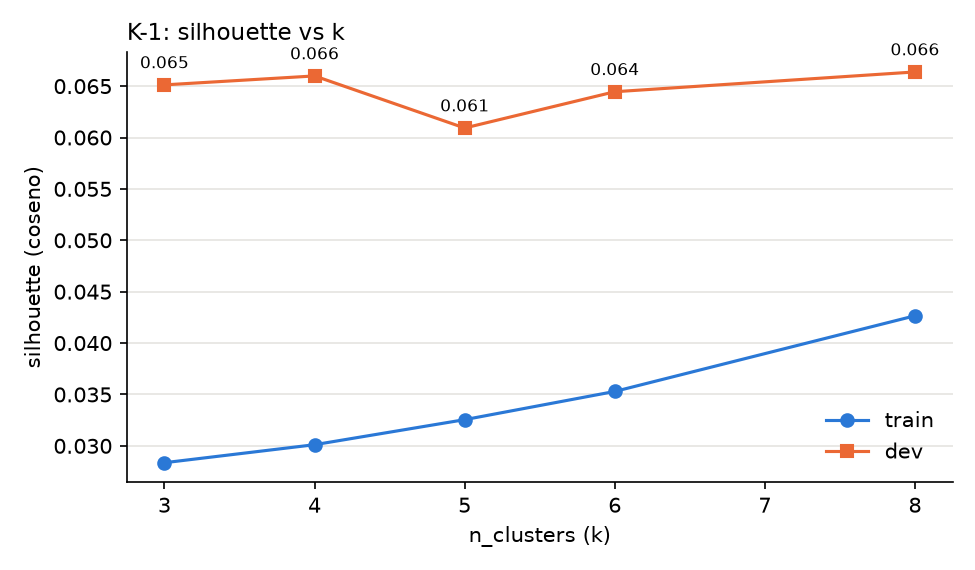
\includegraphics[width=0.68\linewidth]{clustering_silhouette_vs_k.png}
\caption{Silhouette en train y dev para $k \in \{3,4,5,6,8\}$.}
\label{fig:silhouette}
\end{figure}

\subsection{El problema del silhouette entre espacios distintos}
Los bloques K-2 a K-6 aumentaron el silhouette hasta 0.209 (K16: N0, frecuencia,
bigramas, SVD 50). Sin embargo, al revisar las palabras y la contingencia, esos clusters
separaban artefactos de formato (números, notación LaTeX, longitud del abstract), no áreas
de investigación. Su ARI en dev era cercano a 0.04 y su NMI a 0.08. El plan advierte que el
silhouette solo se compara entre configuraciones con el mismo espacio de características;
entre espacios distintos hay que apoyarse en la interpretabilidad. Por eso la cadena
automática por silhouette (K16) no se eligió como configuración final.

\begin{table}[htbp]
\centering
\small
\caption{Ganador automático de cada bloque de clustering.}
\label{tab:kbloques}
\begin{tabular}{@{}llrrr@{}}
\toprule
Bloque & Ganador & $k$ & Silhouette dev & ARI dev\\
\midrule
K-2 (normalización) & K06 (N0) & 3 & 0.0986 & 0.0217\\
K-3 (representación) & K08 (frecuencia) & 3 & 0.1727 & 0.0427\\
K-4 (n-gramas) & K09 (bigramas) & 3 & 0.1873 & 0.0349\\
K-5 (SVD) & K11 (SVD 50) & 3 & 0.2085 & 0.0427\\
K-6 (K-Means) & K16 (random, 20, 500) & 3 & 0.2085 & 0.0427\\
\bottomrule
\end{tabular}
\end{table}

También se probó la representación binaria en K-3 (K17): silhouette dev 0.0477, ARI
$-$0.0038 y estabilidad 0.415. No mejora a TF-IDF (0.0660/0.3755) ni a frecuencia
(0.1727/0.0427); se añadió como complemento para cubrir las tres representaciones.

\subsection{Configuración final}
La configuración final es \textbf{K02}: $k=4$, N2, TF-IDF (1,1), SVD 100,
\code{init="k-means++"}, \code{n\_init=10}, \code{max\_iter=300}, \code{random\_state=0}.
Dentro de su espacio, su silhouette en dev (0.0660) está empatado con el máximo (0.0664) y
sus cuatro clusters son temáticos. Se reajustó con train+dev (425 documentos) y se asignó
test con \code{predict}. Los resultados son: silhouette train+dev \textbf{0.0395}, test
\textbf{0.0829}; ARI test \textbf{0.3719}; NMI test \textbf{0.4860}. La estabilidad con
cinco semillas fue 0.234.

\begin{table}[htbp]
\centering
\small
\caption{Clusters finales: tamaño, palabras principales y documentos representativos.}
\label{tab:clusters}
\begin{tabular}{@{}rp{1.3cm}p{7.3cm}p{3.7cm}@{}}
\toprule
ID & Tamaño & Palabras principales & Representativos\\
\midrule
0 & 192 & training, task, language, token, datum, improve, prompt, target, base, reasoning & 2610.00673, 2609.23449\\
1 & 156 & retrieval, evidence, item, recommendation, query, user, base, agent, language, search & 2609.38473, 2609.37574\\
2 & 113 & video, image, visual, generation, scene, training, physical, benchmark, introduce, representation & 2609.40347, 2610.00812\\
3 & 39 & parameter, training, learn, attention, cost, scale, noise, long, introduce, feature & 2610.00545, 2609.39855\\
\bottomrule
\end{tabular}
\end{table}

\begin{table}[htbp]
\centering
\small
\caption{Contingencia en test: categoría real vs cluster.}
\label{tab:contingencia}
\begin{tabular}{@{}lrrrr@{}}
\toprule
Gold & Cluster 0 & Cluster 1 & Cluster 2 & Cluster 3\\
\midrule
\code{cs.CL} & 13 & 5 & 1 & 0\\
\code{cs.CV} & 4 & 2 & 13 & 0\\
\code{cs.IR} & 1 & 18 & 0 & 0\\
\code{cs.LG} & 12 & 0 & 0 & 6\\
\bottomrule
\end{tabular}
\end{table}

\begin{figure}[htbp]
\centering
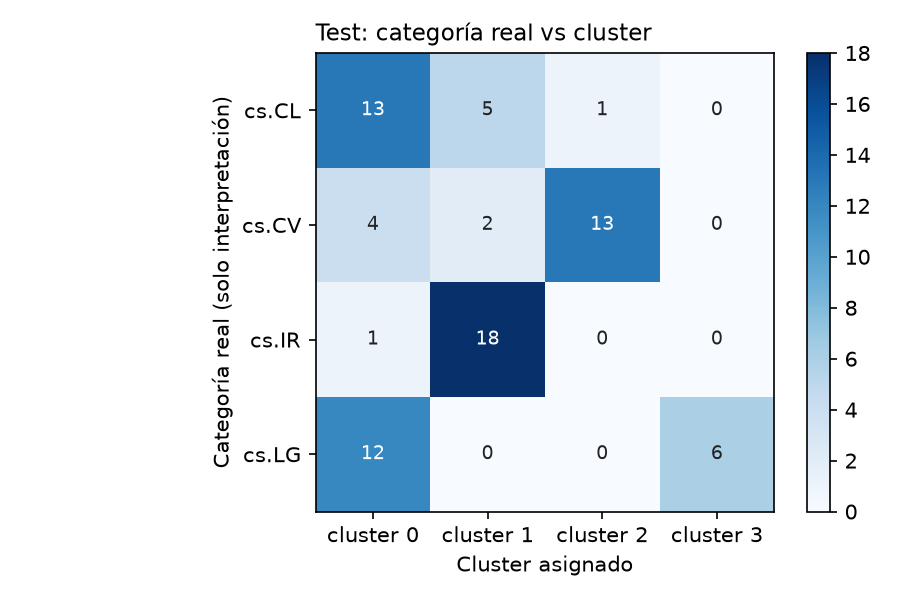
\includegraphics[width=0.58\linewidth]{clustering_contingency_test.png}
\caption{Contingencia en test entre categoría real y cluster.}
\label{fig:contingencia}
\end{figure}

\textbf{Interpretación.} El cluster 1 captura casi todo \code{cs.IR} (18 de 19) y el
cluster 2 casi todo \code{cs.CV} (13 de 19). El cluster 0 mezcla \code{cs.CL} (13) y
\code{cs.LG} (12): es la misma frontera que confunde al clasificador. El cluster 3 es
pequeño (39 documentos) y concentra 6 de los 18 \code{cs.LG}; sus palabras (parameter,
attention, scale, feature) son claramente de ML. El ARI/NMI de test (0.372/0.486) indica
una alineación moderada con las categorías, razonable para un método no supervisado que no
vio las etiquetas. Los tamaños 192/156/113/39 son aceptables; el cluster 3 es el más
pequeño y debería revisarse con más datos.

\begin{figure}[htbp]
\centering
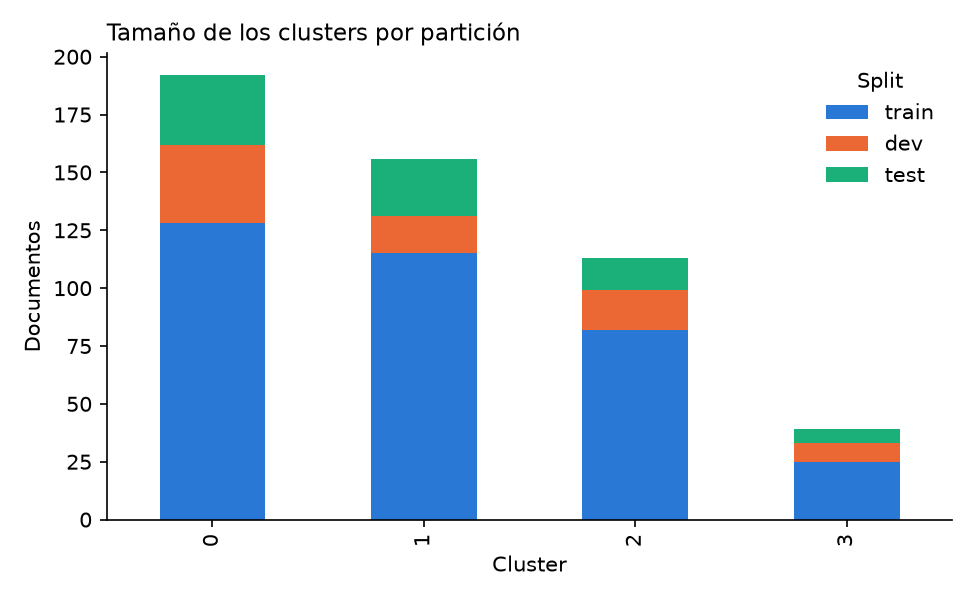
\includegraphics[width=0.72\linewidth]{clustering_sizes.png}
\caption{Tamaño de los clusters por partición.}
\label{fig:tamanos}
\end{figure}

\section{Interfaz de consulta}

La interfaz de línea de comandos permite consultar las métricas y los clusters sin abrir
los notebooks ni los TSV:

\begin{table}[!ht]
\centering
\small
\caption{Comandos de la interfaz.}
\label{tab:cli}
\begin{tabular}{@{}p{8.6cm}p{6.2cm}@{}}
\toprule
Comando & Qué muestra\\
\midrule
\code{python -m src.etapa2.cli metrics} & Métricas de clasificación en dev y test\\
\code{python -m src.etapa2.cli metrics --experiment C02} & Métricas por clase y matriz de confusión de C02\\
\code{python -m src.etapa2.cli clusters} & Tamaños, top-10 palabras y representativos\\
\code{python -m src.etapa2.cli clusters --id 1} & Detalle y documentos representativos del cluster 1\\
\code{python -m src.etapa2.cli experiments --task classification --top 10} & Los 10 mejores experimentos por métrica en dev\\
\bottomrule
\end{tabular}
\end{table}

Además del CLI, se incluye una interfaz web opcional
(\code{python -m src.etapa2.api}, puerto 8001) que clasifica un texto nuevo, muestra
probabilidades y el cluster asignado, y expone las métricas, matrices, clusters y
experimentos. Los modelos finales también se guardan en \code{models/etapa2/}
(\code{classifier\_c02.pkl}, \code{kmeans\_k02.pkl} y \code{metadata.json}) para
reutilizarlos con \code{joblib.load}.

\section{Reproducibilidad}

\subsection{Versiones y semillas}
El entorno se fijó en \code{requirements.txt}: Python 3.14.7, numpy 2.5.4, pandas 3.0.6,
scipy 1.18.1, scikit-learn 1.9.1, spaCy 3.8.16, \code{en\_core\_web\_sm} 3.8.0,
matplotlib 3.11.2, fastapi 0.143.2 y uvicorn 0.54.0. Todas las semillas son 0:
particiones, SVD, modelos y K-Means; la validación cruzada usa
\code{StratifiedKFold(5, shuffle=True, random\_state=0)}. La estabilidad de K-Means usa
las semillas 0--4.

\subsection{Comandos}
Desde la raíz del repositorio, con el entorno activado:

\begin{verbatim}
python -m src.etapa2.labels          # labeled_documents.tsv y splits
python -m src.etapa2.normalization   # cached N0/N1/N2
python -m src.etapa2.classify C-1    # C01-C03
python -m src.etapa2.classify C-2    # C04-C09 (reutiliza C01-C03)
python -m src.etapa2.classify C-3    # C10-C15
python -m src.etapa2.classify C-4    # C16-C21
python -m src.etapa2.classify C-5    # C22-C29
python -m src.etapa2.final           # selección, test y TSV de entrega
python -m src.etapa2.cluster         # K-1 a K-6 y clustering_results.tsv
python -m src.etapa2.cli metrics     # consulta de resultados
\end{verbatim}

Los notebooks \code{06} a \code{13} documentan la Fase 1, los bloques C-1 a C-5, la
Fase 3 y K-Means; los resultados también quedan en \code{experiments.tsv}, en
\code{runs/} y \code{runs\_k/}. La compilación de este informe se hace con
\code{pdflatex Etapa2/informe.tex} (dos pasadas para el índice).

\subsection{Archivos}
\begin{table}[htbp]
\centering
\small
\caption{Entregables generados.}
\label{tab:archivos}
\footnotesize
\begin{tabular}{@{}p{7.0cm}p{7.0cm}@{}}
\toprule
Archivo & Contenido\\
\midrule
\code{data/etapa2/labeled\_documents.tsv} & document\_id, text, label, split, categories\\
\code{data/etapa2/normalized\_variants.tsv} & Caché N0/N1/N2\\
\code{results/etapa2/experiments.tsv} & 46 experimentos (29 de clasificación, 17 de clustering)\\
\code{results/etapa2/}\newline\code{classification\_predictions.tsv} & Predicciones de dev (mejor por modelo) y test\\
\code{results/etapa2/}\newline\code{classification\_metrics.tsv} & Accuracy, macro P/R/F1 por split\\
\code{results/etapa2/}\newline\code{classification\_per\_class.tsv} & Métricas por clase\\
\code{results/etapa2/confusion\_matrices/} & Matrices de confusión en TSV y PNG\\
\code{results/etapa2/error\_analysis.md} & 10 errores de dev explicados\\
\code{results/etapa2/clustering\_results.tsv} & document\_id, split, cluster\_id, configuration\\
\code{results/etapa2/cluster\_summary.tsv} & Tamaño, top-10 palabras y representativos\\
\code{results/etapa2/cluster\_analysis.md} & Selección e interpretación de K-Means\\
\code{models/etapa2/} & classifier\_c02.pkl, kmeans\_k02.pkl y metadata.json\\
\code{src/etapa2/api.py} & Interfaz web opcional (puerto 8001)\\
\code{src/etapa2/} & Módulos de la Etapa II y CLI\\
\bottomrule
\end{tabular}
\end{table}

\section{Limitaciones y conclusiones}

\textbf{Limitaciones.}
\begin{itemize}[leftmargin=1.4em]
\item El corpus es pequeño: 500 documentos y 75 en dev/test. Un documento vale 1.3 puntos;
las diferencias de menos de un punto no son concluyentes.
\item La etiqueta primaria de arXiv es una convención y el cross-listing es alto (43--59\,\%).
Parte del techo de accuracy es estructural.
\item El silhouette de texto es bajo (0.02--0.10) y fácil de inflar con artefactos de
formato; se interpretó junto con las palabras y la contingencia, no como una medida absoluta.
\item La estabilidad de K-Means es moderada (0.234) y el cluster 3 es pequeño (39
documentos); con más datos podría dividirse o fusionarse.
\item El equipo es de dos personas; el reparto de tareas está en el plan de trabajo.
\end{itemize}

\textbf{Conclusiones.}
\begin{itemize}[leftmargin=1.4em]
\item TF-IDF con LogisticRegression y normalización N2 es la mejor combinación: 0.799 en
dev y 0.761 en test. La regularización y el vocabulario compacto son suficientes; no hace
falta SVD.
\item La normalización importa de forma desigual: NB gana 7 puntos con N1, LR gana 4 con
N2 y SVC es casi insensible. No hay una normalización universal.
\item Los bigramas, trigramas y el SVD no mejoran de forma material a LR; en SVC, SVD 50
sube 1.4 puntos en dev pero con CV menor y se añadió después del test, así que no se
seleccionó. La representación TF-IDF ya captura la señal útil con 350 documentos.
\item K-Means encuentra cuatro clusters interpretables (NLP/agentes, IR/recomendación,
visión/vídeo, ML) con ARI 0.372 y NMI 0.486 en test, aunque su silhouette es bajo. El
silhouette más alto no era el más útil: separaba formato, no temas.
\item La clase \code{cs.CL} es la más difícil en dev y test, y su frontera con
\code{cs.LG} es el principal foco de error. El cross-listing explica solo una parte.
\end{itemize}

\clearpage
\appendix
\section{Tabla resumen de experimentos}

\begin{table}[!htbp]
\centering
\small
\caption{Resumen de las configuraciones seleccionadas (detalle completo en
\code{experiments.tsv}).}
\label{tab:resumen}
\footnotesize
\begin{tabular}{@{}>{\raggedright\arraybackslash}p{2.5cm}>{\raggedright\arraybackslash}p{2.0cm}>{\raggedright\arraybackslash}p{2.4cm}>{\raggedright\arraybackslash}p{3.6cm}r>{\raggedright\arraybackslash}p{2.2cm}@{}}
\toprule
Tarea / método & Normalización & Representación & Hiperparámetros & Dev & Notas\\
\midrule
Clasificación / NB & N1 & TF-IDF (1,1) & alpha=0.1; min\_df=2 & 0.7745 & Mejor NB\\
Clasificación / LR & N2 & TF-IDF (1,1) & C=1; min\_df=1 & 0.7993 & Ganador global; test 0.761\\
Clasificación / SVC & N0 & TF-IDF (1,1) & C=10; min\_df=1 & 0.7742 & Mejor SVC\\
Clasificación / LR & N2 & TF-IDF (1,2) & C=1; min\_df=2 & 0.8007 & Empate con C02; no se elige\\
Clasificación / LR & N2 & TF-IDF (1,1)+SVD 50/100/200 & C=10/1; min\_df=2 & 0.7706 & C26-C28 < C02; SVD no ayuda\\
Clasificación / SVC & N0 & TF-IDF (1,1)+SVD 50 & C=10; min\_df=2 & 0.7880 & Dev; CV 0.704; no elegido\\
Clustering / K-Means & N2 & TF-IDF (1,1)+SVD 100 & k=4; k-means++; n\_init=10 & 0.0660 & Silhouette dev; test 0.083\\
Clustering / K-Means & N0 & frecuencia (1,2)+SVD 50 & k=3; random; n\_init=20 & 0.2085 & Silhouette alto, clusters de formato\\
\bottomrule
\end{tabular}
\end{table}

\section{Nota sobre el repositorio}
El proyecto conserva la Etapa I (buscador VSM, 12 configuraciones, benchmark congelado) y
añade la Etapa II en \code{src/etapa2/}, \code{data/etapa2/} y \code{results/etapa2/}. El
corpus, los identificadores y el benchmark de la Etapa I no se modificaron. El informe y el
plan de trabajo están en \code{Etapa2/}.

\end{document}
